\section{Simplicial sets}

\begin{defi}
    The simplicial category $\Delta$ has objects $[n] \coloneqq \{ 0<1<2< \dotsc <n\}$ for $n \geq 0$ and morphisms $\Delta(m,n)\coloneqq \Hom_{\Delta}([m],[n]) \coloneqq \{ f \colon[m] \to [n], \text{order preserving} \}$.
\end{defi}

\begin{defi}
    The \underline{category of simplicial sets} is given by $\Set_{\Delta}=\sSet=\widehat{\Delta}= \Fun(\Delta^{\op},\Set)$.
\end{defi}

\begin{rmk}
    An alternative definiton of a simplicial set $X$ can be given as follows:
    \begin{itemize}
        \item 
            For all $n\geq m$ a set $X_n$ called the \underline{n-simplices} of $X$.
        \item 
            For all $0 \leq i \leq n$ morphisms $d_i\colon X_n \to X_{n+1}$ called the \underline{face maps}.
        \item 
            For all $0 \leq i \leq n$ morphisms $s_i \colon X_n \to X_{n+1}$
            called the \underline{degeneracy maps}.
        \item 
            The face and degeneracy maps satisfy the following identities:
            \[
            \begin{tabular}{ccc}
                 $d_id_j=d_{j-1}d_i$ & $d_is_j=s_{j-1}d_i$ & $d_js_j=\id=d_{j+1}s_j$  
                 \\
                 $i<j$ & $i<j$ & 
                 \\
                 $d_is_j=s_jd_{i-1}$ & $s_is_j=s_{j+1}s_i$
                 \\
                 $i>j+1$ & $i \leq j$
            \end{tabular}
            \]
    \end{itemize}
\end{rmk}

\begin{exmp}
    \begin{enumerate}
        \item 
        For an arbitrary simplicial set we often write
            \[
            \begin{tikzcd}
                X\colon \dotsc 
                &
                X_3
                \arrow[r, altstackar=7]
                &
                X_2
                \arrow[r, altstackar=5]
                &
                X_1
                \arrow[r,altstackar=3]
                &
                X_0
            \end{tikzcd}
            \]
        where the arrows correspond to the face and boundary maps.
        \begin{itemize}
            \item 
            $[0]=\{0\}$
            \item 
            $\relax
            [1]=\{ 
            \begin{tikzcd}
                0
                \arrow[loop left, "id"]
                \arrow[r, "10"]
                &
                1
                \arrow[loop right, "id"]
            \end{tikzcd}
            \}$
            \relax
            \item
            $[2]=\left\{
            \begin{tikzcd}
                &
                1
                \arrow[rd]
                &
                \\
                0
                \arrow[ru]
                \arrow[rr]
                &
                &
                2
            \end{tikzcd}  
            \right\}$
            \item 
            $[3]=\left\{
            \begin{tikzcd}
                &
                1
                \ar[dd]
                \ar[dr]
                &
                \\
                0
                \ar[ru]
                \ar[rr, dashed]
                \ar[rd]
                & 
                &
                2
                \ar[ld]
                \\
                &
                3
                &
            \end{tikzcd}
            \right\}$
        \end{itemize}
    \end{enumerate}
\end{exmp}

\begin{comment}
    
By Yoneda we obtain an isomorphism $\Hom_{\Set_{\Delta}}(\Delta(-,n),X) \isomorphism X_n$. 
Let $x \in X_n$ and let $\Delta^n \coloneqq \Delta(-,n)$ we obtain the following diagram
\[
\begin{tikzcd}
    \Delta^n
    \arrow[rr, "x"]
    \arrow[rd, "\sigma_x"']
    &
    &
    X
    \\
    &
    \Delta^m
    \arrow[ru , "y"']
\end{tikzcd}
\]
\todo{unsure what all is happening here}
\end{comment}

Let $d^i\colon[n-1] \to [n]$ be the unique order preserving injective map not having $i \in [n]$ in its image for all $0 \leq i \leq n$ .
\[
\begin{tabular}{cc}
     \begin{tikzcd}
         \text{[0]}=\{0\}
         \arrow[r, "d^0"]
         &
         \{0 \to \circled{1}\}=[1]
     \end{tikzcd}
     \\
     \begin{tikzcd}
         \text{[}0]=\{0\}
         \arrow[r, "d^0"]
         &
         \{\circled{0} \to 1\}=[1]
     \end{tikzcd}
     \\
     $
     \left\{
     [1]
     =
     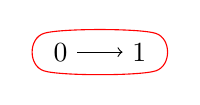
\begin{tikzpicture}[baseline={(0,-0.2)}]
        \node (A) at (0,0) {$0$};
        \node (B) at (1,0) {$1$};
        \draw [->] (A) -- (B);
        \draw [red] plot [smooth cycle] coordinates {(A.north west) (A.south west) (B.south east) (B.north east) };
     \end{tikzpicture}
     \right\}
     \xrightarrow{d^0}
     \left\{
     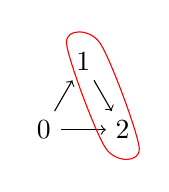
\begin{tikzpicture}[baseline={(0,0.3)}]
        \node (A) at (0,0.866) {$1$};
        \node (B) at (-0.5,0) {$0$};
        \node (C) at (0.5,0) {$2$};
        \draw [->] (A) -- (C);
        \draw [->] (B) -- (A);
        \draw [->] (B) -- (C);
        \draw [red] plot [smooth cycle] coordinates {(A.north west) (A.north east) (C.south east) (C.south west) };
    \end{tikzpicture}
     \right\}=[2]
     $
\end{tabular}
\]
We obtain for any simplicial set $ X $ a diagram
\[
\begin{tikzcd}
    X_n 
    \ar[r, " d_i" ]
    &
    X_{n-1}
    \\
    \Hom_{\SetD} ( \Delta^n , X )
    \ar[u, "\sim" {anchor=south, rotate=90} ]
    \ar[r, " ? \circ d^i_* " ]
    &
    \Hom_{\SetD} ( \Delta^{n-1} , X )
    \ar[u, "\sim" {anchor=south, rotate=90} ]
\end{tikzcd}
\]
and thus for any $ x \in X_n $ a diagram
\[
\begin{tikzcd}
    \Delta^n
    \ar[r , " x " ]
    &
    X
    \\
    \Delta^{n-1}
    \ar[ru]
    \ar[u,"d_*^i"]
    &
    .
\end{tikzcd}
\]
For $ n = 2 $ this looks explicitely as follows
\[
\begin{tikzcd}
    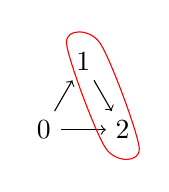
\begin{tikzpicture}
        \node (A) at (0,0.866) {$1$};
        \node (B) at (-0.5,0) {$0$};
        \node (C) at (0.5,0) {$2$};
        \draw [->] (A) -- (C);
        \draw [->] (B) -- (A);
        \draw [->] (B) -- (C);
        \draw [red] plot [smooth cycle] coordinates {(A.north west) (A.north east) (C.south east) (C.south west) };
    \end{tikzpicture}
    \ar[r , "x"]
    &
    X
    \\
    \tikz{
        \node (0) at (-0.5,0) {$0$};
        \node (1) at (0.5,0) {$1$};
        \draw [->] (0) to (1);
    \ar[ru]
    \ar[u]
    }
\end{tikzcd}     
\]
    
\begin{defi}
    The category $\Delta_{\txtbig}$ has as objects the finite non-empty total orders with order preserving maps between them
    \[
    \begin{tabular}{c}
         \begin{tikzcd}
             \Delta
             \arrow[r, hook, shift right]
             &
             \Delta_{\txtbig} 
             \arrow[l, shift right] \ni I = \{ i_0 < i_1 < \dotsc < i_n \}
         \end{tikzcd}      
    \end{tabular}
    \]
\end{defi}

This time we take a closer look at the diagrams that arise from the inclusions of partial orders.

\[
\begin{tabular}{cc}
     \begin{tikzcd}
         \{1\}
         \arrow[r, hook]
         &
         \{0 \to \circled{1}\}
     \end{tikzcd}
     \\
     \begin{tikzcd}
         \{0\}
         \arrow[r, hook]
         &
         \{\circled{0} \to 1\}
     \end{tikzcd}
     \\
     $
     \left\{
     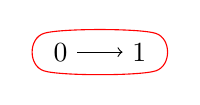
\begin{tikzpicture}[baseline={(0,-0.2)}]
        \node (A) at (0,0) {$0$};
        \node (B) at (1,0) {$1$};
        \draw [->] (A) -- (B);
        \draw [red] plot [smooth cycle] coordinates {(A.north west) (A.south west) (B.south east) (B.north east) };
     \end{tikzpicture}
     \right\}
     \xhookrightarrow{}
     \left\{
     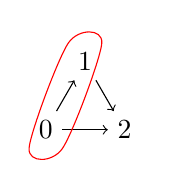
\begin{tikzpicture}[baseline={(0,0.3)}]
        \node (A) at (0,0.866) {$1$};
        \node (B) at (-0.5,0) {$0$};
        \node (C) at (0.5,0) {$2$};
        \draw [->] (A) -- (C);
        \draw [->] (B) -- (A);
        \draw [->] (B) -- (C);
        \draw [red] plot [smooth cycle] coordinates {(A.north west) (A.north east) (B.south east) (B.south west) };
    \end{tikzpicture}
     \right\}
     $
     \\
     $
     \left\{
     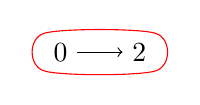
\begin{tikzpicture}[baseline={(0,-0.2)}]
        \node (A) at (0,0) {$0$};
        \node (B) at (1,0) {$2$};
        \draw [->] (A) -- (B);
        \draw [red] plot [smooth cycle] coordinates {(A.north west) (A.south west) (B.south east) (B.north east) };
     \end{tikzpicture}
     \right\}
     \xhookrightarrow{}
     \left\{
     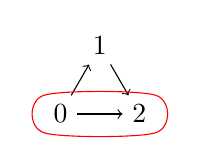
\begin{tikzpicture}[baseline={(0,0.3)}]
        \node (A) at (0,0.866) {$1$};
        \node (B) at (-0.5,0) {$0$};
        \node (C) at (0.5,0) {$2$};
        \draw [->] (A) -- (C);
        \draw [->] (B) -- (A);
        \draw [->] (B) -- (C);
        \draw [red] plot [smooth cycle] coordinates {(B.north west) (B.south west) (C.south east) (C.north east) };
    \end{tikzpicture}
     \right\}
     $
\end{tabular}
\]
These inclusions yield the following poorly organized faces of a square
\[
\begin{tikzcd}
    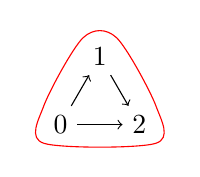
\begin{tikzpicture}
        \node (A) at (0,0.866) {$1$};
        \node (B) at (-0.5,0) {$0$};
        \node (C) at (0.5,0) {$2$};
        \draw [->] (A) -- (C);
        \draw [->] (B) -- (A);
        \draw [->] (B) -- (C);
        \draw [red] plot [smooth cycle] coordinates {(B.north west)  (A.north west) (A.north east) (C.north east) (C.south east) (B.south west) };
    \end{tikzpicture}
    &
    &
    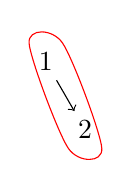
\begin{tikzpicture}
        \node (A) at (0,0.866) {$1$};
        \node (C) at (0.5,0) {$2$};
        \draw [->] (A) -- (C);
        \draw [red] plot [smooth cycle] coordinates {(A.north east)  (C.south east) (C.south west) (A.north west) };
    \end{tikzpicture}
    \ar[ll]
    \\
    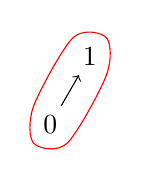
\begin{tikzpicture}
        \node (A) at (0,0.866) {$1$};
        \node (B) at (-0.5,0) {$0$};
        \draw [->] (B) -- (A);
        \draw [red] plot [smooth cycle] coordinates {(B.north west) (A.north west) (A.north east) (A.south east) (B.south east) (B.south west)};
    \end{tikzpicture}
    \ar[u]
    &
    \begin{tikzpicture}
        \node (A) at (0.0) {$1$};
        \draw [red] plot [smooth cycle] coordinates {(A.north west) (A.north east) (A.south east) (A.south west)};
    \end{tikzpicture}
    \ar[l]
    \ar[ru]
    \\
    &
    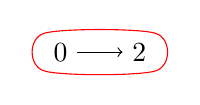
\begin{tikzpicture}[baseline={(0,-0.2)}]
        \node (A) at (0,0) {$0$};
        \node (B) at (1,0) {$2$};
        \draw [->] (A) -- (B);
        \draw [red] plot [smooth cycle] coordinates {(A.north west) (A.south west) (B.south east) (B.north east) };
     \end{tikzpicture}
     \ar[luu]
     &
     \begin{tikzpicture}
        \node (A) at (0.0) {$2$};
        \draw [red] plot [smooth cycle] coordinates {(A.north west) (A.north east) (A.south east) (A.south west)};
    \end{tikzpicture}
    \ar[l]
    \ar[uu]
    \\
    \begin{tikzpicture}
        \node (A) at (0.0) {$0$};
        \draw [red] plot [smooth cycle] coordinates {(A.north west) (A.north east) (A.south east) (A.south west)};
    \end{tikzpicture}
    \ar[uu]
    \ar[ru]
\end{tikzcd} 
\]
which looks applied to a simplicial set as follows
\[
\begin{tikzcd}
    X_2
    \ar[rr]
    \ar[rd]
    \ar[dd]
    &
    &
    X_{\{1 \to 2 \}}
    \ar[rd]
    \ar[dd]
    \\
    &
    X_{\{ 0 \to 2\}}
    \ar[dd]
    \ar[rr]
    &&
    X_{\{2\}}
    \\
    X_{\{0 \to 1 \}}
    \ar[rr]
    \ar[rd]
    &&
    X_{\{1\}}
    \\
    &
    X_{ \{ 0 \} }
\end{tikzcd}
\]
We furthermore have the co-degeneracy maps $ s^i \colon [ n + 1 ] \to [ n ] $ which are the unique order preserving surjective map, that take the value $ i $ twice.
This can be visualised as follows:
\[
\begin{tikzcd}
    0
    \ar[r]
    \ar[d]
    &
    1
    \ar[r]
    \ar[d]
    &
    \dots
    \ar[r]
    &
    i-1
    \ar[d]
    \ar[r]
    &
    i
    \ar[d]
    \ar[r]
    &
    i+1
    \ar[dl]
    \ar[r]
    &
    \dots
    \ar[r]
    &
    n+1
    \ar[dl]
    \\
    0
    \ar[r]
    &
    1
    \ar[r]
    &
    \dots
    \ar[r]
    &
    i-1
    \ar[r]
    &
    i
    \ar[r]
    &
    \dots
    \ar[r]
    &
    n
\end{tikzcd}
\]
and we obtain the following simplex diagram
\[
\begin{tikzcd}
    \Delta^{n+1}
    \ar[r]
    \ar[rd, dashed]
    &
    \Delta^n
    \ar[d, "x"]
    \\
    &
    X
\end{tikzcd}
\]

\begin{exmp}
    Let $ I \in \Set $, we can define the constant simplicial set associated to $ I $, where for all $ n \geq 0 $ we have $ I_n = I $, the faces and degeneracies are the identity functor.    
\end{exmp}

\begin{exmp}
    Let $\mathcal{C}$ be a small category. 
    We define $N(\mathcal{C}) \in \Set_{\Delta}$ as follows. 
    Let $N(\mathcal{C})_0 \coloneqq \Ob(\mathcal{C})$, $N(\mathcal{C})_1=\Mor(\mathcal{C})\colon$ set of morphisms in $\mathcal{C}$ with the face and boundary maps given as follows
    \[
    \begin{tikzcd}
        N ( \mathcal{ C } )_1 
        \ar[r, shift left=1.75ex, "d_0=target"]
        \ar[r, shift right=1.75ex, "d_1=source"']
        &
        N ( \mathcal{ C } )_0
        \ar[l, "s_1"]
    \end{tikzcd}
    \]
    where $ s_1(X) = X \xrightarrow{\id_X} X $ for an $ X \in \Ob ( \mathcal{ C } ) $. Now
    \[
    N ( \mathcal{ C } )_2 =
    \left\{
    \begin{tikzcd}
        &
        f_1
        \ar[rd, "f_{21}"]
        &
        \\
        f_0
        \ar[ru, "f_{10}"]
        \ar[rr, "f_{20}"]
        &&
        f_2
    \end{tikzcd}
    \mid f_{20} = f_{21} \circ f_{10}
    \right\}
    \]
    and we have degeneracies and codegeneracies
    \[
    \begin{tikzcd}
        N ( \mathcal{ C } )_2
        \ar[r, shift left= 2.75ex, "d_0"]
        \ar[r, "d_1" description]
        \ar[r, shift left= -2.75ex, "d_2"']
        &
        N ( \mathcal{ C } )_1
        \ar[l, shift left= - 1.25ex, "s_0"']
        \ar[l, shift left= 1.25ex,"s_1"]
    \end{tikzcd}.
    \]
    Now lastly 
    \[
    N ( \mathcal{ C } )_3 
    =
    \left\{
    \begin{tikzcd}
        & 
        f_1
        \ar[rd, "f_{21}"]
        \ar[dd, "f_{13}" pos=0.7]
        &
        \\
        f_0
        \ar[ru, "f_{10}"]
        \ar[rd, "f_{30}"]
        \ar[rr, dashed, "f_{20}" pos=0.3]
        &&
        f_2
        \ar[dl, "f_{23}"]
        \\
        &
        f_3
        &
    \end{tikzcd}
    \mid \forall i \leq j \leq k 
    f_{kj} \circ f_{ji} = f_{ki}
    \right\}.
    \]
    This gives a functor $ N ( \mathcal{ C } ) \colon \Delta^{\op} \to \Set $ where $ [ n ] \mapsto \Fun( [n] , \mathcal{ C } )$ and thus a simplicial set.
    Note that the nerve has a left adjoint given by the truncation functor.
\end{exmp}

\begin{exmp}
    Let $ X $ be a topological space we define $ \Sing ( X ) $ to be its associated singular simplicial set.
    \begin{itemize}
        \item 
         Let $\Sing ( X )_n \coloneqq \Hom_{\Top} ( \lvert \Delta^n \rvert , X ) $, where $ \lvert \Delta^n \rvert \coloneqq \{ v \in \mathbb{ R }_{\leq 0 }^{n+1}, \lvert \sum_{ i = 0 }^n v_i \rvert = 1 \}$.
        \item 
        For a morphism $ \sigma \colon [ m ] \to [ n ] $ we obtain a morphism $\sigma_* \colon \lvert \Delta^m \rvert \to \lvert \Delta^n \rvert $, where $ \sigma_*( v )_i= \sum_{ j \in \sigma^{-1} ( i ) } v_j$.
    \end{itemize}
    Note that $ \Sing $ has a left adjoint given by the geometric realisation functor.
\end{exmp}

\begin{thm}
    For all $X \in \Set_{\Delta}$ $\lvert X \rvert = \colim_{\substack{([n],x)\in \int_X^\Delta \\
    X\colon \Delta^n \dashv X} }\lvert \Delta^n\rvert$ is a CW complex.
\end{thm}

\begin{defi}
    An element $x$ of simplicial set $X$ is \underline{degenerate} if $x \in \im s_i$ for some $i$.
\end{defi}

\begin{rmk}
    Let $ N ( [ n ] ) = \Hom_{\Cat} ( [ ? ] , [ n ] ) \cong \Hom_{ \Delta } ( [ ? ] , [ n ] ) = \Delta^n $.
    Furthermore for $ \mathcal{ P } $ a poset, let $ N ( \mathcal{ P } )_n = \Hom_{Poset} ( [ n ] , \mathcal{ P } ) $.
    Take now a morphism $ [ n ] \coloneqq \{ 0 < 1 < 2 < \dotsc < n \} \xrightarrow{ \sigma } \mathcal{ P } $ and $ \sigma = ( \sigma_0 , \sigma_1 , \dotsc , \sigma_n ) \in \mathcal{ P }^{n+1} $ such that $ \sigma_0 \leq \sigma_1 \leq \dotsc \leq \sigma_n $, we call this a chain in the poset. 
    Let us now compute $ \Delta^2 = N ( [ 2 ] ) $, we denote the chain $\sigma = ( \sigma_0 , \sigma_1 , \dotsc , \sigma_n )$ by $\sigma_0  \sigma_1  \dotsc  \sigma_n$ in the following table.
    \[
    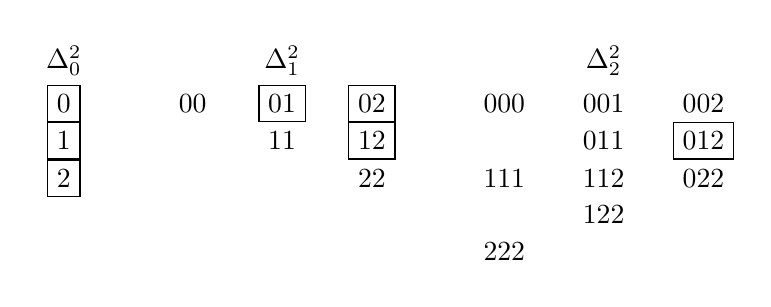
\begin{tikzpicture}
    \matrix [column sep=0.5cm]
    {
    \node{$\Delta_0^2$} ;& ;& ;& \node{$\Delta_1^2$} ;& ;& ;& ;& \node{$\Delta_2^2$} ;&
    \\
    \node[draw] {0}; & ;& \node{00}; & \node[draw]{01}; & \node[draw]{02}; & ;& \node {000}; & \node {001}; & \node {002};
    \\
    \node[draw] {1}; & ;& ;&\node{11};& \node[draw]{12}; & ;& ;& \node {011}; & \node[draw]{012};
    \\
    \node[draw] {2}; & ;& ;& ;& \node{22}; & ;& \node {111};& \node {112};& \node {022}; 
    \\
    ;&;&;&;&;&;&;& \node {122}; &;
    \\
    ;&;&;&;&;&;& \node {222} ;&;&;
    \\
    };
    \end{tikzpicture}
    \]
    The encircled chains correspond to non-degenerate simplices.
    
\end{rmk}

\begin{defi}
    Let $ X \in \SetD $ we write $ \dim X \leq k $ if $ \forall n > k $ we have that $ X_n = X_n^{degeneracies} $.
\end{defi}

We have a functor that goes from simplicial sets to simplicial groups and is similar to the free functor from set to abelian groups.
\[
\begin{tikzcd}
    X \in \SetD = \Fun ( \Delta^{\op}, \Set ) 
    \ar[d, "\mathbb{Z}"]
    \\
    \Ab_{\Delta} = ( \Fun ( \Delta^{ \op } , \Ab ) )
\end{tikzcd}
\]
We write $ ( \mathbb{ Z } X )_n = \mathbb{ Z } \langle X_n \rangle $.
Let now $ Y \in \Ab_{\Delta} $ be a simplicial abelian group, we associate to it a chain complex $ C ( Y ) \in \Ch_{\geq 0 } ( \Ab ) $, where $C ( Y )_n \coloneqq Y_n$ and the differential is given as 
\begin{align*}
    C ( Y )_n 
    &\to 
    C ( Y )_{ n -1 }
    \\
    x 
    &\mapsto
    \partial ( x ) = \sum_{i = 0}^n (-1)^i d_i ( x ).
\end{align*}

\begin{rmk}
    \begin{enumerate}
        \item 
        If we now take $ X \in \Top $ we can take $ \Sing ( X ) \in \SetD $ then $ \mathbb{ Z } \Sing ( X ) \in \Ab_{\Delta} $ and then $ C ( \mathbb{ Z } \Sing ( X ) ) \in \Ch_{\geq 0}$ with its $n$-th component being given by $ \mathbb{ Z } \langle \Hom_{ \Top } ( \lvert \Delta^n \rvert , X ) \rangle \in \Ab $.
        This complex is called the Moore complex and its associated homology groups give the integral singular homology $ H_* ( X ; \mathbb{ Z } ) $ of the space $ X $.
        Furthermore we can define the homology groups $ H_n( Y , A )$ of a simplical set $ Y $ with coefficients in an abelian group $ A $ to be the homology groups $ H_n ( \mathbb{ Z } Y \otimes A )$ of the chain complex $ \mathbb{ Z } Y \otimes A $.

        \item 
        Let $ \mathcal{ A } $ be an exact category. 
        Then $\mathcal{ A } $ has an associated category $ Q \mathcal{ A } $ with objects those of $ \mathcal{ A } $ and arrows given by equivalence classes of diagrams 
        \[
            \bullet \twoheadleftarrow \bullet \rightarrow \bullet
        \]
        where both arrows are parts of exact sequences of $ \mathcal{ A } $, and composition is represented by pullback. 
        Then $ K_{i-1} ( \mathcal{ A } ) \coloneqq \pi_i \lvert BQ\mathcal A \rvert $ defines the $ K $-groups of $ \mathcal{ A } $ for $  i \geq 1 $; in particular $ \pi_i \lvert B Q \proj ( R ) \rvert = K_{i-1} ( R )$, the $ i^{th}$ algebraic $K$-group of the ring $ R $, here $ \proj ( R ) $ denotes the category of finitely generated projectives over $ R $.
    \end{enumerate}
\end{rmk}

\begin{defi}
    The normalized Moore chain of $ Y $ is the chain complex with components $ \overline{C} ( Y )_n \coloneqq \bigcap_{ i = 1 }^n \ker d_i $ and differentials $ \partial_n = d^n_0 $.
\end{defi}

\begin{thm}(Dold-Kan Correspondences)
    Let $ \Delta \to \Ch_{ \geq 0 } $ be given by $ [n ] \mapsto \overline{C} ( \mathbb{ Z } ) \Delta^n $, then there exists an adjunction.
    \[
    \begin{tikzcd}
        \Bar{C}\colon \Ab_{\Delta}
        \ar[r, shift left]
        &
        \Ch_{ \geq 0 }( \Ab ) : DK 
        \ar[l , shift left, "\sim"]
    \end{tikzcd}
    \]
\end{thm}

\subsection{Exercises}

\begin{Exercise}
        Show that the functor $ \widehat{ \Delta }  \to \SetD $ which remembers only the face and degeneracy maps and is the identity on morphisms is an isomorphism of categories. 
        In particular,
         \begin{itemize}
             \item 
             show that the functor is well defined by showing that the co-face and co-degeneracy maps satisfy the cosimplicial identities.
             \begin{align*}
                 d^jd^i &= d^i d^{j-1} \quad \text{ if } i < j
                 \\
                 s^j s^i &= s^i s^{j+1} \quad \text{ if } i \leq j
             \end{align*}
             \qquad
             $
             s^j d^i=
             \begin{cases}
                 d^i s^{j-1} &\text{ if } i < j 
                 \\
                 \id &\text{ if } i \in \{ j , j + 1 \}
                 \\
                 d^{i-1} s^j &\text{ if } i > j = 1
             \end{cases}
             $
             Recall that the co-face maps $ d^i \coloneqq d_n^i $ and co-degeneracy maps $ s^i \coloneqq s_n^i $ are defined as follows for each $ n \in \mathbb{ N }_+ $ respective $ n \in \mathbb{ N }_0 $ and $ 0 \leq i \leq n $.  
             \begin{align*}
                 d^i = d_n^i \colon [ n - 1 ] &\to [ n ]
                 \\
                 k &\mapsto 
                 \begin{cases}
                     k & \text{ if } k < i 
                     \\
                     k+1 & \text{ if } i \leq k 
                 \end{cases}
             \end{align*}
             \quad
             \begin{align*}
                 s^i = s_n^i \colon [ n n 1 ] &\to [ n ]
                 \\
                 k &\mapsto 
                 \begin{cases}
                     k & \text{ if } k \leq i 
                     \\
                     k-1 & \text{ if } i < k 
                 \end{cases}
             \end{align*}
        
             \item  
             For the inverse, show that a morphism $ \sigma \colon [m] \to [n] $ in $ \Delta $ can be uniquely written as
            \[
                \sigma 
                =
                d_n^{i_s}
                \circ d_{ n - 1 }^{i_{s-1}} 
                \circ 
                \dotsm 
                \circ
                d_{ n - s + 1 }^{i_1}
                \circ
                s_{ m - t }^{j_1}
                \circ 
                \dotsm
                \circ
                s_{ m - 2 }^{ j_{t-1}}
                \circ 
                s_{ m - 1 }^{j_t}
            \]
            with $ 0 \leq i_1 < i_2 < \dotsm < i_s \leq n $ and $ 0 \leq j_1 < j_2 < \dotsm < j_t < m $ and $ n-s = m-t $.
        \end{itemize}
    \end{Exercise}
    
    \begin{Exercise}
        
    Fix $ n \in \mathbb{ N }_+ $.
    Define the simplicial subset $ \partial \Delta^n \subseteq \Delta^n $ by
    \[
        \partial \Delta^n ( [ m ] ) \coloneqq \{ \sigma \colon [ m ] \to [ n ] \text{ non-surjective } \}
    \]
    and similarly, define for $ 0 \leq k \leq n $ the simplicial subset $ \Lambda_k^n \subseteq \partial \Delta^n $ by
    \[
        \Lambda_k^n( [ m ] ) \coloneqq \{ \sigma  \in \partial \Delta^n ( [ m ] ) \mid \sigma ( [ m ] ) \neq [ n ] \setminus \{ k \} \}.
    \]
    \begin{enumerate}[label=(\alph*)]
        
        \item 
        Confirm that the above are indeed simplicial subsets.
    
        \item 
        Show one of the following 
        \begin{itemize}
        
            \item 
            $ \partial \Delta $ is the smallest simplicial subset of $ \Delta^n $ such that $ \{ d_n^i \mid 0 \leq i \leq n \} \subseteq \partial \Delta^n ( [ n - 1 ] ) $.
    
            \item 
            $\Lambda_k^n$ is the smallest simplicial subset of $ \Delta^n $ such that $ \{ d_n^i \mid 0 \leq i \leq n \wedge i \neq k \} \subseteq \Lambda^n_k ( [ n - 1 ] )$.
            
        \end{itemize}
    
    Recall that we may view $ \Delta $ as a category of posets, so that we may compute the nerve of ( subsets of ) $ [ n ] $ as partially ordered set.
    Moreover, we may associate to $ [ n ] $ the category $ \Sub_* ( [ n ] ) $ of non-empty proper full subcategories, i. e. $ [ n ] \notin \Sub_* ( [ n ] ) $, and morphisms given by inclusions.
    Similarly, we define for $ k \in [ n ] $ the full subcategory $ \Sub_*^k ( [ n ] ) \coloneqq \{ k \in E \in \Sub_* ( [ n ] ) \subseteq  \Sub_* ( [ n ] )$.
    
        \item 
        Show one of the following.
    
        \begin{enumerate}
            \item 
            \[
                \partial \Delta^n
                \cong 
                \bigcup_{ E \in \Sub_* ( [ n ] ) } N ( E ) \coloneqq 
                \colim_{ E \in \Sub_* ( [ n ] ) } N ( E ) 
            \]
    
            \item 
            \[
                \partial \Delta^n
                \cong
                \bigcup_{ E \in \Sub_* ( [ n ] ) } N ( E ) \coloneqq 
                \colim_{ E \in \Sub_* ( [ n ] ) } N ( E ) 
            \]
        \end{enumerate}
    
        \item 
        Justify the notation $ \bigcup $.
        
    \end{enumerate}
\end{Exercise}

\begin{Exercise}
    Let $ \Delta_{ \leq n } $ be the full subcategory of $ \Delta $ of the elements $ [ 0 ] , [ 1 ] , \dotsc , [ n ] $.
    The inclusion $ \iota_n \colon \Delta_ { \leq n } \to \Delta $ induces a truncation functor $ \tr_n \coloneqq ( \iota_n )^* \colon \Set_{ \Delta } \to \widehat{ \Delta_ { \leq n } } $.

    \begin{enumerate}[label=(\alph*)]
        
        \item 
        Show that $ \tr_n $ admits both a left and a right adjoint, $ \sk_n \dashv \tr_n \dashv \cosk_n $, which are both fully faithful.
    
        \item 
        Deduce that we have an adjunction $ \bold{sk_n} \coloneqq \sk_n \circ \tru_n \dashv \cosk_n \circ\tru_n \eqqcolon \bold{ cosk_n } $ of endofunctors of $ \SetD $.
        
    \end{enumerate}
    
    The essential image of $ \sk_n $ are called the $ n $-skeletal simplicies while the essential image of $ \bold { cosk_n } $ are the $ n $-coskeletal simplices.
    
    \begin{enumerate}[label=(\alph*), resume]
        \item 
        Show that a simplicial set $ X $ is $ n $-skeletal if and only if 
        
        $ \tru_n \colon \Hom_{ \SetD } ( X , - ) \to \Hom_{ \widehat{ \Delta{ \leq n }}} ( \tru_n X , \tru_n ( - ) ) $ is an isomorphism of functors.
    
        \item 
        Show that a simplicial set $ Y $ is $ n $-coskeletal if and only if
        
        $ \tru_n \colon \Hom_{ \Set_\Delta } ( - , Y ) \to \Hom_{ \widehat{ \Delta_{ \leq n }} } ( \tru_n ( - ) , \tru_n Y ) $ is an isomorphism of functors.
    \end{enumerate}
\end{Exercise}

\begin{Exercise}
    \begin{enumerate}[label=(\alph*)]
         \item 
         Show that a map $ F \colon X  \to N ( \mathcal{ C } ) $ to the nerve of a category $ \mathcal{ C } $, is completely determined by a map $ u \colon X_1 \to \Mor ( \mathcal{ C } ) $ such that 
         \begin{enumerate}
             \item 
             for all $ x \in X_0 $ we have that $ u ( s_0 ( x ) ) $ is an identity and 
    
             \item 
             for any $2$-simplex $ \sigma \in X_2 $ we have that $ u ( d_1 ( \sigma ) ) = u ( d_0 ( \sigma ) ) \circ u ( d_2 ( \sigma ) )$.
         \end{enumerate}
    
         \item 
         Deduce that the nerve of a category is 2-coskeletal.
    
         \item 
         Conclude that the nerve $ N \colon \Cat \to \SetD $ is fully faithful.
    \end{enumerate}
\end{Exercise}

\begin{Exercise}
    Consider the functor $ \Op \colon \Delta \to \Delta $ which is the identity on objects and for $ \sigma : [ n ] \to [ m ] $
    \[
        \Op ( \sigma ) ( i ) 
        \coloneqq
        m - \sigma ( n - i )
    \]
    Let $ ( - )^{ \op } \coloneqq \Op^* \colon \SetD \to \SetD $ be the corresponding involution of the category of simplicial sets.
    
    \begin{enumerate}[label=(\alph*)]
        \item 
        Show that $ \Op $ is a well defined involution.
    
        \item 
        For a simplicial set $ X $, describe the face and degeneracy maps of $ X ^{ \op } $.
    
        \item 
        Show that for a category $ \mathcal{ C } $ we have an isomorphism $ N ( \mathcal{ C }^{\op} ) \cong N ( \mathcal{ C } )^{\op} $.
    
        \item   
        Show that for a topological space there is an isomorphism $ \Sing ( X ) \cong \Sing ( X )^{ \op } $ for the singular complex of $ X $.
    \end{enumerate}
\end{Exercise}